\begin{section}{Literature Review}

\begin{subsection}{Evolution of Trade Between China and ASEAN}

China’s accession to the WTO in 2001 marked an important new opportunity to forge closer economic ties around the world. The idea to adopt a ACFTA between ASEAN member states and China was first voiced at the ASEAN-China summit on 6 November 2001. On 4 November 2002, China and ASEAN Countries signed the New Framework Agreement on Comprehensive Economic Cooperation (hereafter named "the Agreement") which formed the legal basis for the creation of the ACFTA (\cite{asean_2002_1}). 

\begin{figure}[H]
	\centering
	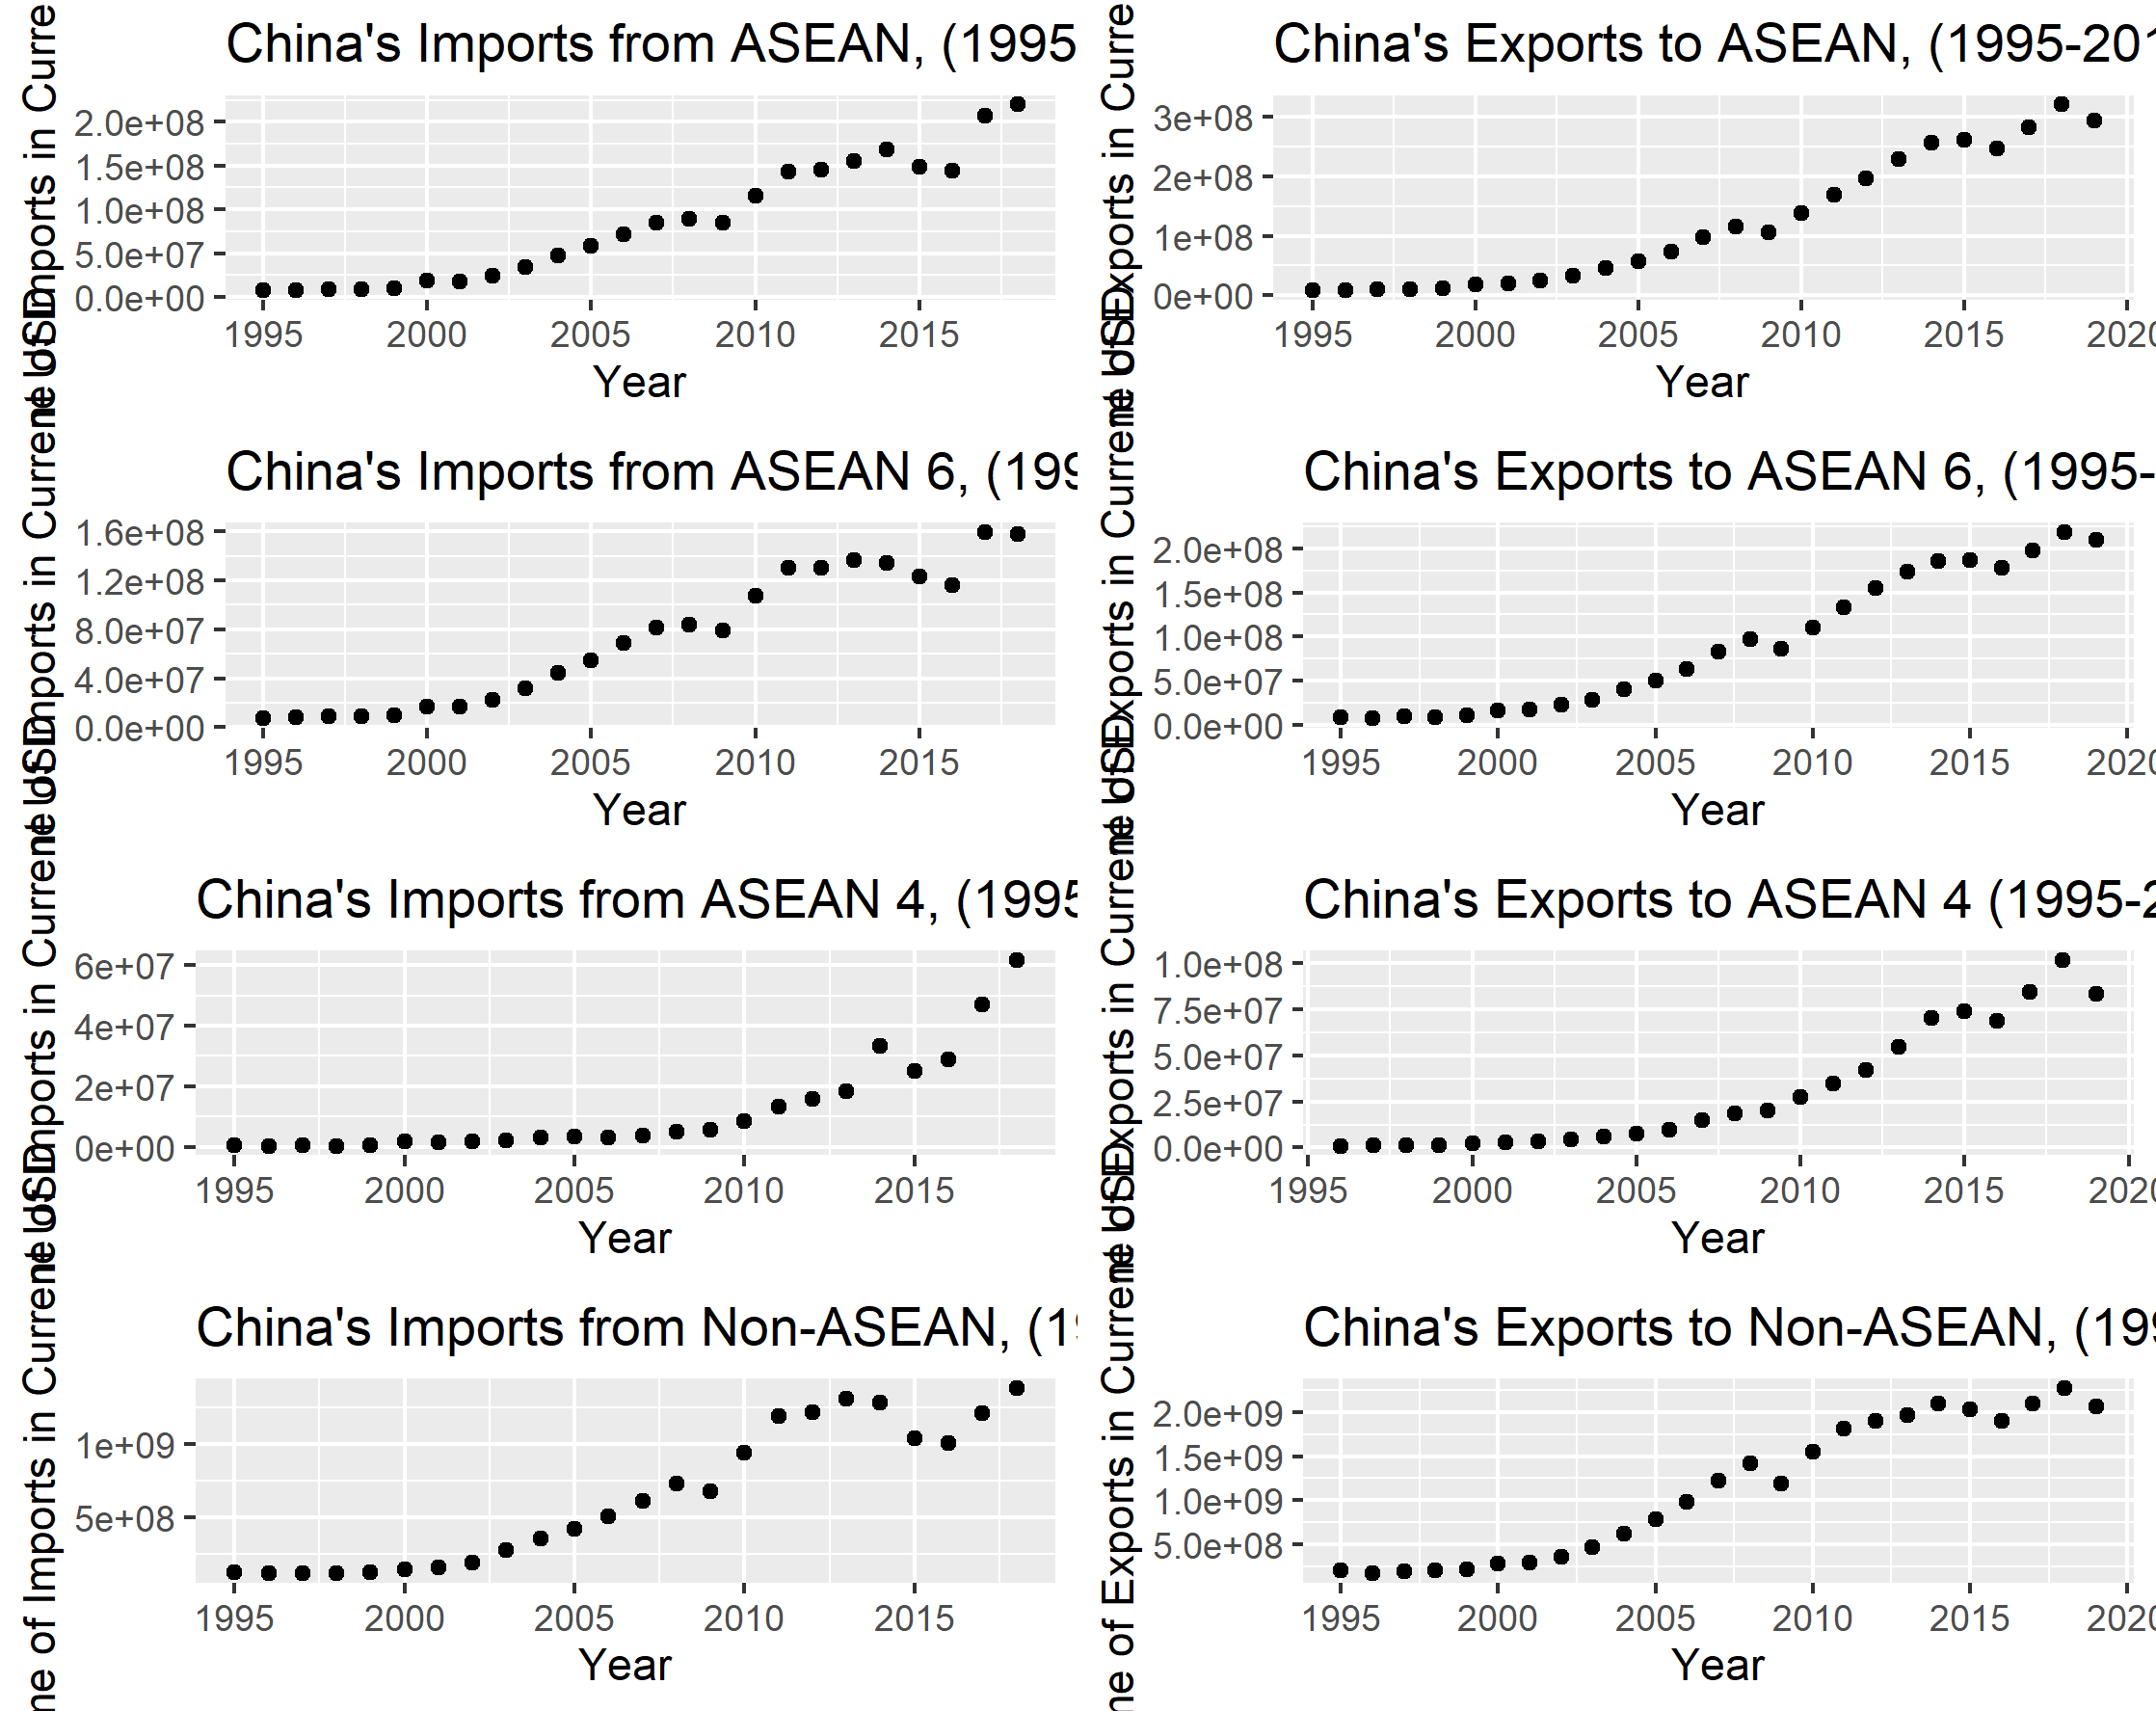
\includegraphics[width=\textwidth]{figure_1.png}
	\caption{\small{Evolution of Exports and Imports of ASEAN Countries with China over Time. Grouped by ASEAN6 and ASEAN4 Countries. \textit{Source:} UN Comtrade Import Data Retrieved in \cite{cepii-data_2022}.}}
	\label{fig_1}
\end{figure}

In order to interpret the evolution of trade flows shown in \autoref{fig_1}, it is worthwhile to consult the Agreement. Policymakers aimed at stimulating trade between ASEAN and China through the reduction of both tariff- and non-tariff barriers. 

A potentially substantial part of the rise in trade flows can be associated with the tariff reduction and elimination program as described in Article 3 of the Agreement (\cite{asean_2002_1}). Article 3 foresees a gradual reduction in tariffs along two major categories \footnote{See \cite{asean_2002_4}, as well as \cite{asean_2002_2} and \cite{asean_2002_3} for details.} \autoref{tab_1} shows that, depending on whether products were listed in the Normal or the Sensitive Track, applied MFN tariffs were to be reduced at different paces, between two different sets of countries. The first set of countries were the earlier ASEAN 6 member states Brunei, Indonesia, Malaysia, Philippines, Singapore and Thailand. The second set of countries were Cambodia, Lao, Myanmar and Vietnam ("ASEAN 4"). As seen, for ASEAN 6 and China, products listed in the Normal Track were to reduce or eliminate their respective applied MFN tariff rates gradually over a period from 1 January 2005 to 2010. In the case of the four newer ASEAN members, the period was from 1 January 2005 to 2015. ASEAN 6 and China were to reduce the applied MFN tariff rates of tariff lines placed in their respective Sensitive Track to 20\% not later than 1 January 2012. These tariff rates were then subsequently reduced to 0-5\% not later than 1 January 2018. Cambodia, Lao, Myanmar and Vietnam were to reduce the applied MFN tariff rates of tariff lines placed in their respective Sensitive Lists to 20\% not later than 1 January 2015. These tariff rates were then subsequently reduced to 0-5\% not later than 1 January 2020. 

\begin{table}[H]
\centering
\begin{tabular}{ccccc} 
\hline
\multicolumn{1}{l}{} & \multicolumn{1}{l}{}   & \textbf{Normal Track }                                                                                        & \multicolumn{2}{c}{\textbf{Sensitive Track}}                                                                                                \\ 
\cline{3-5}
\multicolumn{2}{c}{\textbf{Trade Partners}}   & \begin{tabular}[c]{@{}c@{}}\textbf{Applied MFN Tariff }\\\textbf{to be reduced}\\\textbf{until }\end{tabular} & \begin{tabular}[c]{@{}c@{}}\textbf{Applied MFN Tariff }\\\textbf{to be reduced }\\\textbf{to at least (\%)}\end{tabular} & \textbf{until }  \\ 
\hline
\textbf{ASEAN 6}     & \textbf{China}         & 1 January 2010                                                                                                & 20                                                                                                                       & 1 January 2012   \\
\textbf{ASEAN 6}     & \textbf{China}         & \multicolumn{1}{l}{}                                                                                          & 5                                                                                                                        & 1 January 2018   \\
\textbf{ASEAN 4}     & \textbf{China}         & 1 January 2015                                                                                                & 20                                                                                                                       & 1 January 2015   \\
\textbf{ASEAN 4}     & \textbf{China}         & \multicolumn{1}{l}{}                                                                                          & 5                                                                                                                        & 1 January 2020   \\
\hline
\end{tabular}
\caption{\small{ACFTA Tariff Liberalisation Along Two Different Country Groups and Products. \textit{Source:} \cite{asean_2002_1}.}}
\label{tab_1}
\end{table}

From the annexes of \cite{asean_2002_4} we infer that due to the vast heterogeneity of the tariff policy packages across countries, products and time, attributing trade flow effects to their respective tariff reduction episodes is beyond our scope. While this might sound discouraging at first, there is also another side of the medal. In addition to the tariff reductions, the Agreement foresees a row of further fields of economic integration (\cite{asean_2002_1}). For instance, the parties have agreed on gradually eliminating non-tariff barriers starting 1 January 2005. Furthermore, negotiators took into consideration the different stages of development among ASEAN member states: special conditions in connection to export facilitation were adopted in more recent member states such as Cambodia, Lao and Vietnam, in order for them to catch up in terms of domestic capacity, efficiency and competitiveness.

Given this heterogeneity in the trade policy package, our aim is to grasp the trade effects of the Agreement as a whole. In our gravity regressions, we account for this by using dummy variables that are meant to capture the entirety of trade liberalisation policies associated with the ACFTA.

\end{subsection}

\begin{subsection}{Trade Creation and Trade Diversion: Using Gravity}

\begin{subsubsection}{Ex-Post Assessment of Regional Trade Agreements: The Gravity Model}

A common practice, we believe that starting with a gravity model is best to get an idea about the effects of a regional trade agreement. The structural gravity model describes how bilateral trade flows of country $i$ to country $j$ in period $t$ react to changes in the level of bilateral “freeness” of trade (\cite{mvzj_2019}). Thus, the main advantage of the structural gravity model is that it delivers a tractable framework for trade policy analysis in a multi-country environment. Following \cite{ypl_2016}, we motivate our choice by briefly explaining the structural gravity which our specifications rely upon. 

\begin{equation}\label{eq_1}
    Trade_{ij}=\frac{Y_{i}E_{j}}{Y}\Big(\frac{t_{ij}}{\Pi_{i}P_{j}}\Big)^{1-\sigma}
\end{equation}

The theoretical structural gravity equation \ref{eq_1} governs bilateral trade flows. It can be conveniently decomposed into two terms: (i) a size term $\frac{Y_{i}E_{j}}{Y}$, (ii) and a trade cost term $\Big(\frac{t_{ij}}{\Pi_{i}P_{j}}\Big)^{1-\sigma}$.
\bigskip
\\
(i) The \textit{size term} consists of the world GDP ($Y$), the GDP of countries $i$ and $j$ ($Y_{i}$ and $E_{j}$), respectively. Thus, it carries some very useful information regarding the relationship between country size and bilateral trade flows.
\bigskip
\\
(ii) The \textit{trade cost term} captures the total effects of trade costs that drive a wedge between realized and frictionless trade. The trade cost term consists of three components:
\begin{itemize}
\item Bilateral trade cost between partners $i$ and $j$, $t_{ij}$.
\item The structural term $P_{j}$ , coined by \cite{avw2003} as inward multilateral resistance represents importer $j$’s ease of market access.
\item The structural term $\Pi_{i}$, defined as outward multilateral resistance by \cite{avw2003}, measures exporter $i$’s ease of market access.
\end{itemize}

Given the multiplicative nature of the structural gravity equation \ref{eq_1}, and assuming that it holds in each period of time $t$, it is possible to log-linearize it and expand it with an additive error term:
\begin{equation}\label{eq_2}
   \ln{Trade_{ijt}}=\ln{E_{jt}}+ \ln{Y_{it}}-\ln{Y_{t}}+(1-\sigma)\ln{t_{ijt}}-(1-\sigma)\ln{P_{jt}}-(1-\sigma)\ln{\Pi_{it}}+\varepsilon_{ijt}
\end{equation}
The standard practice suggested in the literature is to proxy for the
bilateral trade cost term, $(1-\sigma)\ln{t_{ijt}}$, by using a series of observable variables most of which have become standard covariates in empirical gravity specifications \cite{ypl_2016}:
\begin{equation}\label{eq_3}
(1-\sigma)\ln{t_{ijt}}=\beta_{1}\ln{Dist_{ij}} + \beta_2 Lang_{ij} + \beta_3 Contig_{ij} + \beta_4RTA_{ijt}+\varepsilon_{ijt}
\end{equation}

Inserting equation \ref{eq_3} into equation \ref{eq_2} yields equation \ref{eq_4} below. 

\begin{equation}\label{eq_4}
\begin{aligned}
   \ln{Trade_{ijt}} &=\ln{E_{jt}}+ \ln{Y_{it}}-\ln{Y_{t}}+\beta_{1}\ln{Dist_{ij}} + \beta_2 Lang_{ij} + \beta_3 Contig_{ij} + \beta_4RTA_{ijt}\\
   &-(1-\sigma)\ln{P_{jt}}-(1-\sigma)\ln{\Pi_{it}}+\varepsilon_{ijt}
\end{aligned}
\end{equation}

\end{subsubsection}

\begin{subsubsection}{Theory: Trade Creation and Trade Diversion using Gravity}

\textit{Trade creation and diversion effects}. The effects of an RTA can be captured by using dummy variables. \cite{carrere_2006} decomposes trade effects of RTAs into intra-bloc trade effects and extra-bloc trade effects. In there, intra-bloc trade refers to trade between members, while extra-bloc trade relates to trade activities between members and non-members, including FTA exports to non-members and imports from non-members. Altogether, there are three FTA dummy variables to capture trade creation and trade diversion effects: an intra-bloc FTA dummy ($\gamma_{1}$), an extra-bloc export dummy ($\delta_{1}$) and an extra-bloc import dummy ($\delta_{2}$). \autoref{tab_2} presents the possible trade effects considering these three FTA dummy variables.

\begin{table}[H]
\centering
\begin{tabular}{lccc} 
\hline
                                             & \textbf{Intra-bloc trade}                                                         & \multicolumn{2}{c}{\begin{tabular}[c]{@{}c@{}}\textbf{Extra-bloc trade}\\ \end{tabular}}                                                                                 \\ 
\cline{2-4}
                                             & \begin{tabular}[c]{@{}c@{}}\textbf{Trade between }\\\textbf{members}\end{tabular} & \begin{tabular}[c]{@{}c@{}}\textbf{Export to }\\\textbf{non-members}\end{tabular} & \begin{tabular}[c]{@{}c@{}}\textbf{Import from }\\\textbf{non-members}\end{tabular}  \\ 
\hline
\multicolumn{1}{c}{\textbf{Trade creation}}  & $\gamma_1 > 0$                                                                    & $\delta_1 > 0$                                                                    & $\delta_2 > 0$                                                                       \\
\multicolumn{1}{c}{\textbf{Trade diversion}} & $\gamma_1 < 0$                                                                    & $\delta_1 < 0$                                                                    & $\delta_2 < 0$                                                                       \\
\hline
\end{tabular}
\caption{\small{Potential Magnitudes: Trade Creation and Trade Diversion Effects}}
\label{tab_2}
\end{table}

\textit{Third-country effects.} Similar to the concept of interdependence of RTAs introduced in \cite{bbm2014}, the trade volume of countries belonging to an independent RTA can be affected by this independent RTA and existing alternative bilateral trade agreements. The effects of the remaining RTAs are decomposed into the "Own-FTA effect" and "Cross-FTA effect" (see \autoref{fig_3}). Take ACFTA as an example; these third-country effects are made up of both the trade flows between single ACFTA member countries and their respective third-RTA partner countries (“Own-ACFTA effect”) as well as countries that are part of an RTA which is neither the set of either ACFTA nor ACFTA partner countries (”Cross-ACFTA effect”). 

\begin{figure}[H]
	\centering
	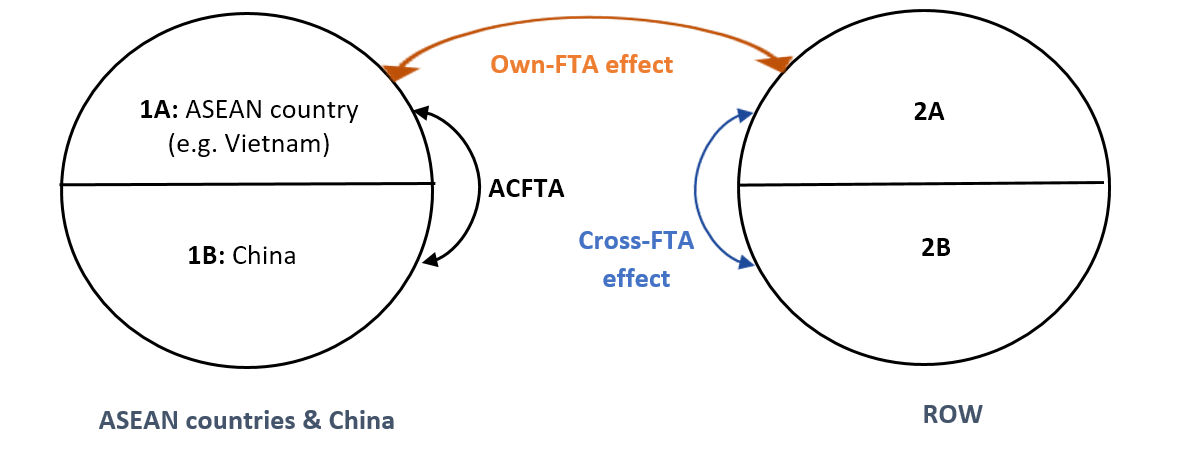
\includegraphics[width=\textwidth]{figure_3.png}
	\caption{\small{Trade Creation and Trade Diversion: Own-FTA effects and Cross-FTA effects.}}
	\label{fig_3}
\end{figure}

\end{subsubsection}

\begin{subsection}{Empirical Review: Trade Creation, Trade Diversion or Both?}

\begin{subsubsection}{Data}

\begin{figure}[H]
	\centering
	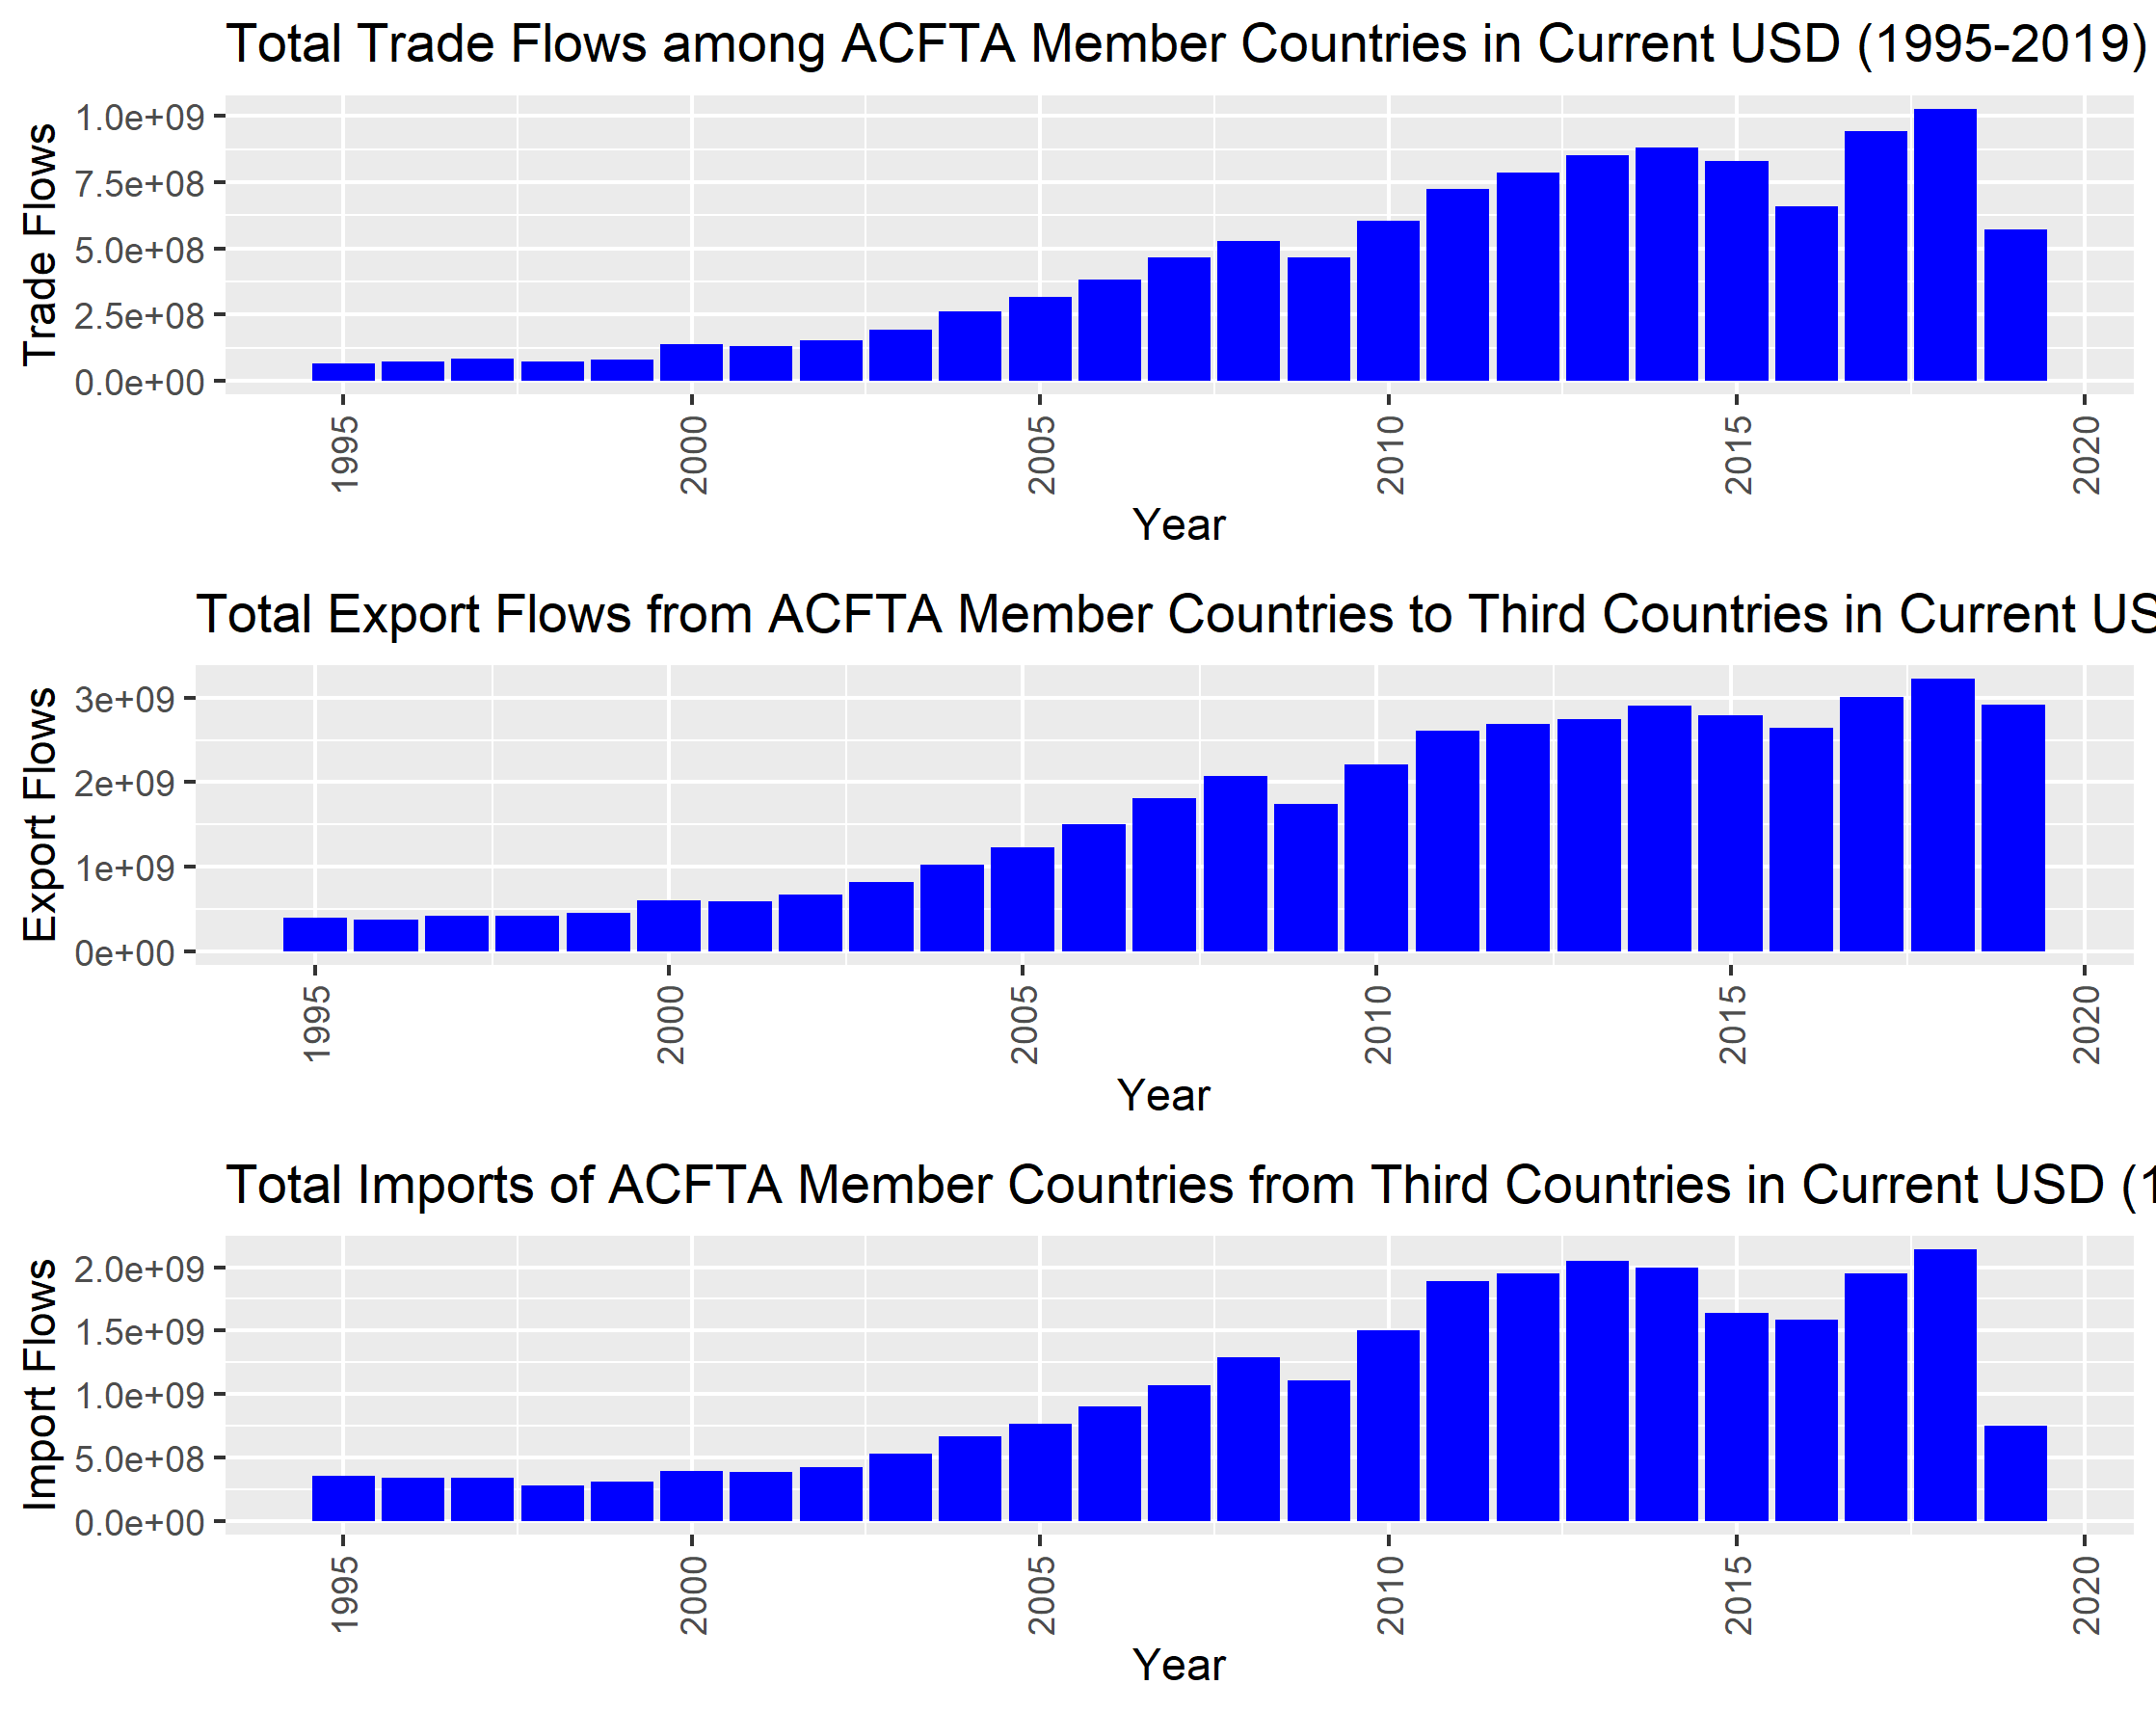
\includegraphics[width=\textwidth]{figure_2.png}
	\caption{\small{Evolution of Trade Flows within ACFTA as well as Ex- and Imports from and to ACFTA. \textit{Source:} \cite{cepii-data_2022}. Missing BACI Data were Replaced by UN Comtrade Import Data.}}
	\label{fig_2}
\end{figure}

\end{subsubsection}

\begin{subsubsection}{Survey of the Literature}

This part intends to provide a brief survey of those papers closest to our methodology and regional trade integration episode. Conceptually, our aim to obtain trade integration effects goes back to \cite{viner1950}. Extending Viner's core idea of different trade effects, depending on whether a country is part of an integration episode or not, we model three different sets of FTA dummy variables representing trade creation and diversion effects in terms of export and import.\footnote{It was \cite{endoh1999} who first formalized this idea.} As our study intends to add to the grand debate around Vinerian trade creation and trade diversion in the literature on the ACFTA, we focus on studies that explore the trade impacts of ACFTA on ASEAN member countries, China and their respective third trading partners. 

\cite{smz2014}'s structural gravity framework intends to capture trade creation and trade diversion effects of ACFTA. They test their model on a sample of 31 countries over the period from 1995 to 2010 using UNCTAD export data for agricultural and manufactured goods and within manufactures for chemical products, as well as for machinery and transport equipment. Distinguishing between agricultural and manufacturing goods, they acknowledge the fact that the agreements involve different tariff-reduction schedules over time\footnote{Different provisions apply for agricultural goods (Early Harvest Products) and for manufacturing goods (Normal Track of the Agreement, see Section 2.1)}, and such can have distinctive effects on trade flows. Zooming in allows to examine sectors of particular importance for the overall trade effects.

A second study that uses a structural gravity framework is \cite{wla_2021}. The authors investigate the effects of exports from ACFTA to the 79 countries that together make up 95\% of ASEAN's export volume. In order to differentiate whether the formation of ACFTA has accelerated trade among both ASEAN member countries and non-ASEAN members, they employ three different dummy variables.  This allows them to separate between three different effects of trade creation and diversion, measured by export and import flows both within \textit{ACFTA} countries and between \textit{ACFTA} and \textit{Non-ACFTA} countries (see also \cite{carrere_2006}). First, the authors regress log trade flows on the dummies, controlling for GDP, population, language, distance and border contiguity, landlocked and islands in a pooled OLS regression. Second, they estimate the same specification with random effects. Finally, employing a battery of time-invariant fixed effects, the authors regress log trade flows on the dummies and log GDP and log population. 

\end{subsubsection}


\begin{subsubsection}{Hypotheses}
Our specifications and literature at hand, we expect overall trade creation due to ACFTA. We expect this both within the ACFTA bloc and between the ACFTA bloc and its partners. Hence, our first hypothesis is that $\gamma_1$, $\delta_1$ and $\delta_2$ are positive in sign for ACFTA and its third export and import partners (see \autoref{tab_2}).
\pagebreak
Our second hypothesis is placed within the context of trade diversion and robustness. \cite{ksy2018} hypothesize that the formation of a trade agreement has negative spillover effects in terms of less trade in non-member countries. We include an additional dummy $otherRTA$ that covers all FTAs apart from the ACFTA. This helps us to compare the effect of the ACFTA formation to all other trade creation or diversion effects from 2003 onwards. We expect the trade creation effect of the ACFTA during the examined period to be more pronounced than the trade creation effect for all other FTAs.
\end{subsubsection}

\end{subsection}

\end{subsection}

\end{section}
